\documentclass[12pt,a4paper]{report}

\usepackage[utf8]{inputenc}
\usepackage[T1]{fontenc}
\usepackage[english]{babel}
\usepackage[top=1cm,bottom=2cm,left=1cm,right=1cm]{geometry}
%\usepackage{url}
%\usepackage{fancyhdr}
\usepackage{sectsty}
\usepackage{wrapfig}
\usepackage{titlesec}
\usepackage{setspace}
\usepackage{graphicx}
\usepackage{lmodern}
\usepackage{url}
\usepackage{amsmath}
\usepackage{amssymb}
\usepackage{mathrsfs}
\usepackage{fancyhdr}
\usepackage{gensymb}
\usepackage{enumerate}
\usepackage{caption}
\usepackage{hyperref} % Créer des liens et des signets 
\usepackage[cc]{titlepic}
\usepackage{listing}

\title{
\rule{15cm}{1pt} \\
\Large {\bfseries Sensation and percetion} \\
\Large {\bfseries Assignement 2}\\
\rule{15cm}{1pt}}
\author{Sami Sellami}

\titlepic{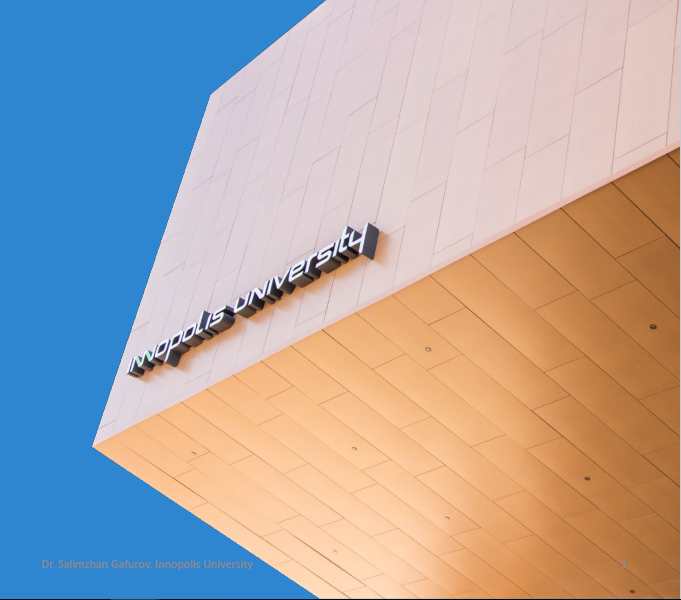
\includegraphics[width=15cm]{Innopolis_image.png}} 
\date{\today}

\begin{document}
\pagenumbering{arabic}
\setcounter{page}{1}
\setcounter{secnumdepth}{1}
	
\fontfamily{ptm}\selectfont

\maketitle

\titlelabel{\thetitle)\quad}
\titlespacing{\chapter}{0cm}{0cm}{0cm}
\titlespacing{\section}{0.2cm}{0cm}{0cm}

THE SOURCE CODE IS ATTACHED TO THE PRESENT FILE 

\subsection{TASK 1: Case 4 Estimating propoer trajectory using kalman filter}

After uploading the dataset we can plot our dataset:

\begin{center}
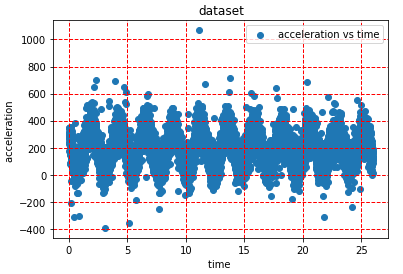
\includegraphics[width=8cm]{Capture1.png}
\captionof{figure}{Acceleration in respect of time}
\end{center}

For estimating the proper trajectory we implement a code in python for filtering our data using kalman filter
This is the code 
\begin{verbatim}
def kalman (data):
    x=data_frame.y
    sigmaEta=x.std()
    sigmaPsi=1    
    x_opt=[]
    x_opt.append(x[0])    
    e_opt=[]    
    e_opt.append(sigmaEta)    
    K=[]
    K.append(1)
    for t in range (x.size-1):
        e_opt.append(math.sqrt( (sigmaEta**2 *(e_opt[t]**2 +sigmaPsi**2) ) 
        / (sigmaEta**2 + e_opt[t]**2 + sigmaPsi**2) )  )
        K.append(e_opt[t+1]**2/sigmaEta**2)    
        x_opt.append(K[t+1]*x[t+1]  + (1-K[t+1])*x_opt[t])
    return x_opt   
\end{verbatim}

And we obtain the following graph after filtering:

\begin{center}
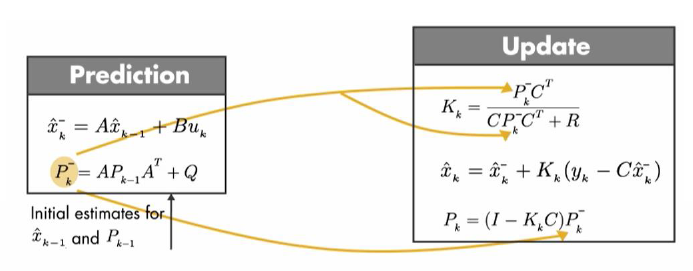
\includegraphics[width=8cm]{Capture2.png}
\captionof{figure}{Acceleration in respect of time after using kalman filter}
\end{center}

\subsection{TASK 2: Camera Calibration}
We take 30 pictures of our chess board and we compute the algorithm for camera calibration in PYTHON:

\begin{center}
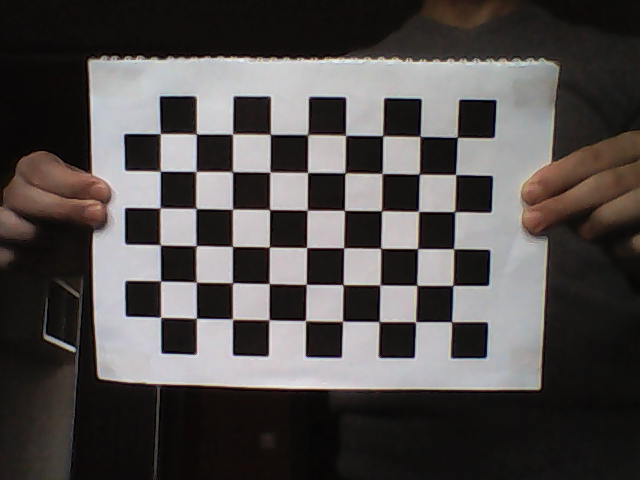
\includegraphics[width=8cm]{Capture6.png}
\captionof{figure}{Image of the ChessBoard}
\end{center}

we need at least 10 test patterns for camera calibration, we use the function  "cv.findChessboardCorners()" to find pattern in the chess board and  " cv.drawChessboardCorners()" to draw the pattern 

\begin{center}
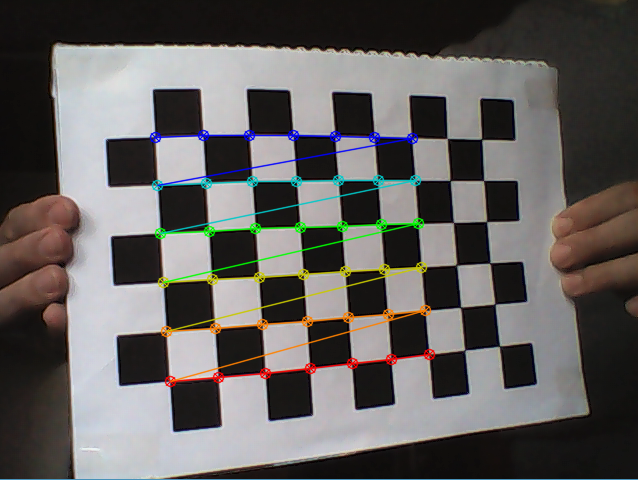
\includegraphics[width=7cm]{Capture7.png}
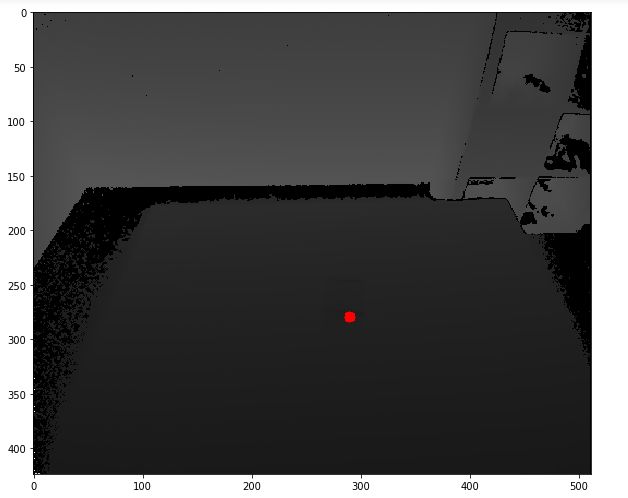
\includegraphics[width=7cm]{Capture8.png}
\captionof{figure}{Images with pattern drawn in it}
\end{center}

Now we can calibrate the camera and extract the intrinsic and extrinsic parameters:

IntrinsicParameters$  =\left[\begin{array}{ccc}  06884456 &  0   &      266.9266647 \\
   0     &    824.39349912 & 218.14799475 \\
   0    &       0   &        1        \end{array}\right]$

The funciotn calibrateCamera return extrinsic parameters in the form of rotation vector and translation vector, the rotation is a  vector formed of the euler angles representing the rotation, to obtain the rotation matrix, we use the code linked in python file to converst Euler angles to rotation matrix

The extrinsic parameters depend on the positon of the chess board, so for each image we have different extrinsic paramters, we are going to represent one matrix for one postion of the chess board:
 
 
$$Rotation Matrix  =\left[\begin{array}{ccc} -0.9789908 &  0.00383985 & -0.20386826\\
        0.10467765& -0.848553  & -0.51865248\\
       -0.17498457 &-0.52909646 & 0.83032364 \end{array}\right]$$

$$Translation Vector_{scale1}   =\left[\begin{array}{ccc} 3.72721863\\
       3.12062999\\
       18.41341474 \end{array}\right]$$

We have to multiply the result by the size of the chess board square which is $2.4mm$ since our algorithm give us a reuslt in the scale of size of chess board square

$$Translation Vector   =\left[\begin{array}{ccc}8.945324712\\
       7.489511975\\
       44.192195376 \end{array}\right]$$
And finally:

$$ExtrinsincParameters  =\left[\begin{array}{cccc} -0.9789908 &  0.00383985 & -0.20386826& 8.945324712\\
        0.10467765& -0.848553  & -0.51865248&7.489511975\\
       -0.17498457 &-0.52909646 & 0.83032364&44.192195376 \end{array}\right]$$

We take a picture of a cup at about 20cm and we propose to estimate its dimensions using the calibrated camera:

\begin{center}
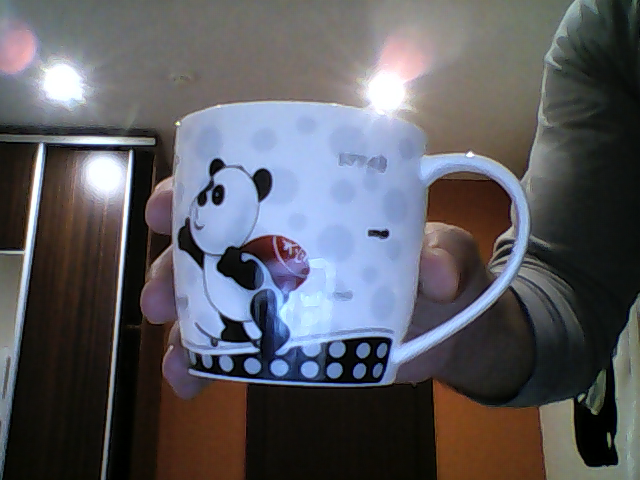
\includegraphics[width=8cm]{Capture9.png}
\captionof{figure}{Images of a cup}
\end{center}

The dimensions of the cup can be computed using the expression above comprising the intrinsic and extrinsic matrices and the coordinates of the cup in the image plane:

\begin{center}
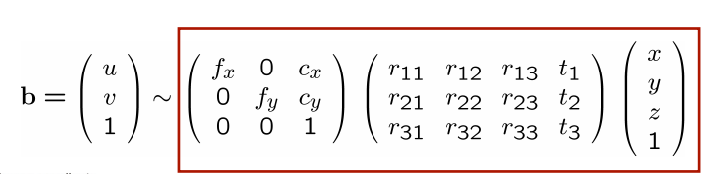
\includegraphics[width=10cm]{Capture10.png}
\end{center}

We know that $t_{1}=t_{2}=0$, $t_{3}=200mm$ and we suppose that there is no rotation, and knowing the resolution of the camera we can obtain $x, y, z=200$ 
$$x=x_{image}*resolution/size_{image}=640*4.5/11.5$$
$$y=y_{image}*resolution/size_{image}=480*5/8.5$$

and we can calculate $X,Y$


\subsection{TASK 3: Case 17 Fundamental matrix and disparity map}

We have a dataset which contains left and right images from a scene, the task is to use 8 points algorithm in order to find the fundamental matrix:

First we have to find a minimum of 8 corresponding points in both images, for that we use key point detection technique namely the function "load stereoPointPairs" in MATLAB and we obtain the following plot:

\begin{center}
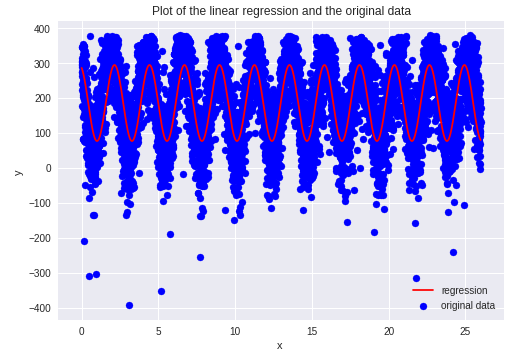
\includegraphics[width=17cm]{Capture3.png}
\captionof{figure}{matched points in the stereo image}
\end{center}
 
The following plot show the stereo image ater conserving only inliers 
\begin{center}
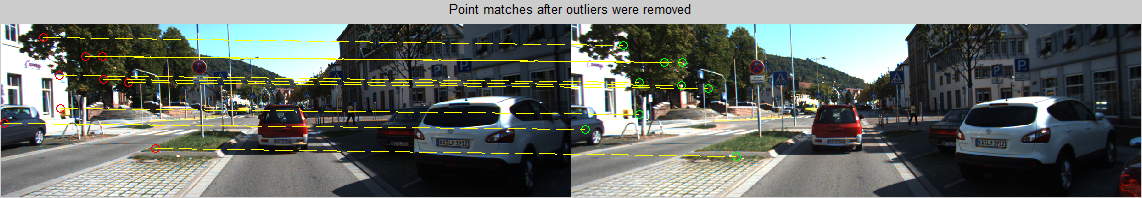
\includegraphics[width=17cm]{Capture4.png}
\captionof{figure}{matched points in the stereo image after outliers removal}
\end{center}

After that we can compute the fundamental matrix :
$$F= \left[ \begin{array}{ccc}
4,70534018328790e-06	& -0,000360913108080483	& 0,0348275622082616\\
0,000364453646511181	& 3,36531699206132e-06	& -0,0937286010924828\\
-0,0425517566149795	& 0,0993083850885704	& 0,989164068589324 \end{array} \right]$$

\subparagraph{Disparity map:}
We use matlab and a diparity range of $[-6, 10]$ to compute the disparity map and we obtain the following plot:
\begin{center}
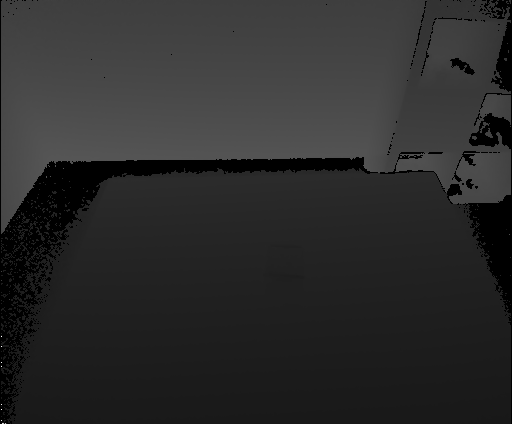
\includegraphics[width=17cm]{Capture5.png}
\captionof{figure}{Disparity map}
\end{center}



\end{document}	
